\chapter{Development of OXC Framework\label{chap:impl}}
The oxc framework is still ongoing. Latest codes can be found 
in github\footnote{https://github.com/YIYAYIYAYOUCHENG/linux}.
The oxc framework is not a scheduler. Although it cooperates with
different scheduling classes, its pure responsibility is managing 
the distribution of CPU power, which depends on modular schedulers 
to use it for scheduling tasks. Under oxc framework, we also call
oxc scheduling as oxc control since it is utilized to control CPU 
bandwidth reservation.

\section{Implementation of ox container structure}
An ox container \texttt{struct oxc\_rq}, listing~\ref{lst:oxc_rq}, 
is defined in Linux kernel. In \texttt{struct oxc\_rq} there 
are fields for reserving bandwidth from a CPU using CBS rules. 
In the following context, an \texttt{struct oxc\_rq} instance is 
also called an ox container, container, or oxc runqueue for the 
same meaning. An oxc runqueue also corresponds to a constant 
bandwidth server in CBS theory. 
The CPU reservation for oxc runqueues follows the implementation 
of CBS reservation for a RT runqueue in IRMOS framework. 

\begin{lstlisting}[language=C, 
		caption={The ox container : \texttt{struct oxc\_rq}},
                        label={lst:oxc_rq}]
struct oxc_rq {
	unsigned long oxc_nr_running;
	inx oxc_throttled;
	u64 oxc_deadline;
	u64 oxc_time;
	u64 oxc_runtime;
	ktime_t oxc_period;
	struct hrtimer oxc_period_timer;
	raw_spin_lock oxc_runtime_lock;
	struct rq rq_;
	struct rq *rq;
	struct rb_node rb_node;
};
\end{lstlisting}

\begin{itemize}
\item \texttt{oxc\_nr\_running} is the number of oxc tasks enqueued in 
		the container's local runqueue. We say these tasks work 
		in the ox container.
\item \texttt{oxc\_throttled} is set when an ox container runs out of
		its budget in a period.	Here ''throttled'' is a 
		convention inherited from RT throttling and 
		maps to the suspended state of a CBS. 
\item \texttt{oxc\_deadline} is current deadline of this ox container,
		which is a server in CBS theory.
\item \texttt{oxc\_time} is currently consumed budget in a period.
\item \texttt{oxc\_runtime} and \texttt{oxc\_period} are CBS parameters:
		\texttt{oxc\_runtime} is maximum budget and 
		\texttt{oxc\_period} is the period.
\item \texttt{oxc\_period\_timer} is timer which will activate at recharging
		time. If at some point, the value of \texttt{oxc\_time} is 
		larger than the value of \texttt{oxc\_runtime}, then
		the ox runqueue will be throttled and 
		its timer will be set to fire, at the 
		current deadline, \texttt{oxc\_deadline}, 
		to recharge the container.
\item \texttt{oxc\_runtime\_lock} guarantees that the update of an ox 
		container's reservation parameters (\texttt{oxc\_runtime} 
		and \texttt{oxc\_period}) and internal state 
		(\texttt{oxc\_time} and \texttt{oxc\_deadline}) happen
		in a consistant way.
\item \texttt{rq\_} is the local runqueue of the ox container.
\item \texttt{rq} points to a per CPU runqueue and its CPU is where the 
		ox container reserves bandwidth from.
\item \texttt{rb\_node} is used to put an ox runquneue in a red black tree.
		All oxc runqueues reserve bandwidth from the same CPU
		are sorted in a red-black tree. In this tree, an ox 
		container's \texttt{oxc\_deadline} value is used to order 
		nodes.
\end{itemize}
For each CPU, there is a red-black tree which stores all oxc runeueues that
reserve bandwidths in this CPU and orders them with their current deadline.
The oxc runqueue with earliest deadline is stored in the leftmost node. 
This tree is called the edf tree and is defined in 
\texttt{struct oxc\_edf\_tree}.

\begin{lstlisting}[language=C, caption={The EDF tree}]
struct oxc_edf_tree {
	struct rb_root rb_root;
	struct rb_node *rb_leftmost;
};
\end{lstlisting}
The pointer \texttt{rb\_leftmost} helps fast access to the earliest deadline
ox container in a CPU.

An ox container is responsible for reserving bandwidth from a CPU.
Another data structure \texttt{struct hyper\_oxc\_rq} is defined to 
reserve bandwidth from multiple CPUs. A \texttt{struct hyper\_oxc\_rq}
instance is called a hyper ox container. 

\begin{lstlisting}[language=C, caption={The hyper ox container}]
struct hyper_oxc_rq {
	cpumask_var_t cpus_allowed;
	struct oxc_rq ** oxc_rq;
};
\end{lstlisting}
\begin{itemize}
\item \texttt{cpus\_allowed} specifies the CPUs that are used to reserve 
				bandwidth.
\item \texttt{oxc\_rq} is an array of (pointers to) ox containers to 
		reserve bandwidth from CPUs identified in 
		\texttt{cpus\_allowed}.
\end{itemize}

\section{Extensions on original data structures\label{sec:extention}}
Several new data structures have been imported in the kernel that will
involve with Linux schedulers , yet the interfaces defined in 
\texttt{struct sched\_class} are kept unmodified. Extensions are added 
in some original data structures in order to merge newly defined data 
structures in the system. Such extensions are not complex.

\begin{lstlisting}[language=C, caption={Extensions on \texttt{struct rq}}]
struct rq {
	...
	int in_oxc;
	struct oxc_edf_tree oxc_edf_tree;
};
\end{lstlisting}
Two fileds are added in runqueue structure. The \texttt{in\_oxc} is 
used to distinguish per CPU and ox container runqueue.
As the name says, for an ox container's local runqueue, its 
\texttt{in\_oxc} field is set. And \texttt{oxc\_edf\_tree} in a 
per CPU runqueue is the edf tree for a CPU to keep and sort ox
containers.

The kernel configuration option \texttt{CONFIG\_CGROUP\_SCHED} is required
by the oxc framework. This option allows to create arbitrary task groups
using the "cgroup" pseudo filesystem. In current implementation of oxc 
framework, reservation is made for tasks in a control group. Tasks in a 
cgroup is represented by the \texttt{struct task\_group} structure. And 
extensions also happen inside it.

\begin{lstlisting}[language=C, 
			caption={Extensions on 
					\texttt{struct task\_group}}]
struct task_group {
	...
	struct hyper_oxc_rq *hyper_oxc_rq;
	int oxc_label;
};
\end{lstlisting}
Because tasks in a cgroup can span multiple CPUs, \texttt{struct task\_group}
is a good place to put the hyper ox container. If a task group has been
allocated CPU bandwidths through oxc control, then this task group runs 
inside a hyper ox container, and its \texttt{hyper\_oxc\_rq} points 
to that hyper container; otherwise, this field is NULL. As before,
a task group inside a hyper oxc is called an oxc task group.
There are three types of oxc task groups: an oxc group whose father
is not an oxc task group; an oxc task group whose father is an oxc group
with a different hyper ox container; an oxc task group with the same hyper
ox container as its father. The \texttt{oxc\_label} field is used to 
differ them. For non oxc task group, this field is not utilized.

When oxc scheduling is enabled in the kernel, there are two kinds of tasks
in the system: oxc tasks and non oxc tasks. To difference between them
is that oxc tasks work is (or will be) enqueued in an ox container's local 
runqueue and non oxc tasks work with a per CPU runqueue. So, from a task, 
its associated runqueue can be tracked according to the scheduling route 
in figure~\ref{fig:scheduling_route_oxc} or~\ref{fig:oxc_task_no_tg}.
As long as the runqueue is found, given its \texttt{in\_oxc} field, the 
status of this runqueue and the task can both be fixed. Consider that 
the question ''is that an oxc task?'' happens frequently in the framework, 
a \texttt{is\_oxc\_task} field is added in \texttt{struct task\_struct} for 
efficient recognition of an oxc task.

\begin{lstlisting}[language=C, caption={\texttt{is\_oxc\_task} field in 
						\texttt{struct task\_struct}}]
struct task_struct {
	int is_oxc_task;
	...
};
\end{lstlisting}
When a task runs in an ox container, this new field is set.

\section{To direct a task to a per ox container runqueue\label{sec:redir}}

In section~\ref{sec:design_oxc_scheduling}, we show the scheduling routes
when there exists oxc scheduling in a system. This section will introduce
the details on how to build these scheduling routes.

\subsection{To build the scheduling route in mainline Linux}

In order to schedule a task in a per oxc runqueue, the first thing is to 
associate this task with the local runqueue of an oxc. To understand this,
let's first see how the system associates a task to a runqueue in mainline 
Linux, where there is only per CPU runqueues. This is done through
the method \texttt{set\_task\_rq}.

\begin{lstlisting}[language=C, label={lst:set_task_rq},
	caption={To associate tasks with a per CPU runqueue in mainline Linux}]
void set_task_rq(struct task_struct *p, unsigned int cpu)
{
#ifdef CONFIG_FAIR_GROUP_SCHED
        p->se.cfs_rq = task_group(p)->cfs_rq[cpu];
        p->se.parent = task_group(p)->se[cpu];
#endif

#ifdef CONFIG_RT_GROUP_SCHED
        p->rt.rt_rq  = task_group(p)->rt_rq[cpu];
#endif
}
\end{lstlisting}

As demonstrated in list~\ref{lst:set_task_rq}, codes inside 
\texttt{set\_task\_rq} build up the front part of the scheduling route 
when \texttt{CONFIG\_FAIR\_GROUP\_SCHED} and 
\texttt{CONFIG\_RT\_GROUP\_SCHED} are set.
When RT or CFS task group scheduling is enabled, each task is then directed 
to its task group. In mainline Linux, the second part of a scheduling route
only directs a task group to the per CPU runqueues. Such paths are connected 
when the task group is created. Figure~\ref{fig:tg_creation} shows the hint how 
a task group joins the scheduling route during its creation. In addition, now 
we know that a scheduling route is built backwards from an runqueue end.

\begin{figure}[htbp]
        \centering
        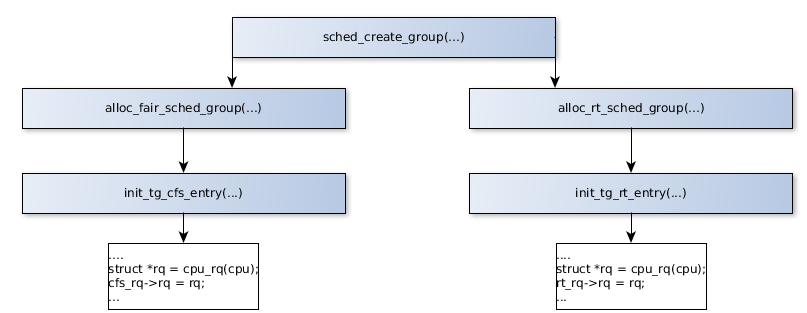
\includegraphics[width=\textwidth]{images/tg_creation}
        \caption{The creation of a task group in original Linux}
        \label{fig:tg_creation}
\end{figure}
In case that task group scheduling is not enabled, recall the scheduling path
where the \texttt{task\_rq} leads a task to its per CPU runqueue directly.

\subsection{To build the scheduling route in oxc enabled Linux}

Now, we have seen the point when a task or task group joins the scheduling 
route in mainline Linux. These points are still time to fill elements in 
scheduling routes, figure \ref{fig:scheduling_route_oxc} and 
\ref{fig:oxc_task_no_tg}, after oxc runqueues are imported in Linux.

Previously, the \texttt{set\_task\_rq} method does not deal with the task 
that is not in a RT or CFS task group. This is because for tasks without 
group scheduling, the scheduling route \texttt{task\_rq} is utilized.
However, \texttt{task\_rq} does not work for an oxc task to locate the
per container runqueue. The functionality of \texttt{set\_task\_rq} is
then extended to care about tasks without group scheduling. 

\begin{lstlisting}[language=C, 
        caption={The extended \texttt{set\_task\_rq}}]
void set_task_rq(struct task_struct *p, unsigned int cpu)
{
        struct task_group *tg = task_group(p);

#ifdef CONFIG_FAIR_GROUP_SCHED
        p->se.cfs_rq = tg->cfs_rq[cpu];
        p->se.parent = tg->se[cpu];
#else
        if(!tg->hyper_oxc_rq)
                p->se.cfs_rq = &cpu_rq(cpu)->cfs;
        else
                p->se.cfs_rq = &tg->hyper_oxc_rq->oxc_rq[cpu]->rq_.cfs;
#endif

#ifdef CONFIG_RT_GROUP_SCHED
        p->rt.rt_rq  = tg->rt_rq[cpu];
        p->rt.parent = tg->rt_se[cpu];
#else
        if(!tg->hyper_oxc_rq)
                p->rt.rt_rq = &cpu_rq(cpu)->rt;
        else
                p->rt.rt_rq = &tg->hyper_oxc_rq->oxc_rq[cpu]->rq_.rt;
#endif
        if (rq_of_task(p)->in_oxc == 1)
                p->is_oxc_task = 100;
        else
                p->is_oxc_task = 0;
}
\end{lstlisting}
                                                  
When task group scheduling is enabled, there is no difference for setting a 
task's runqueue in both
the mainline Linux and oxc enabled Linux. The interesting part happens when 
task group scheduling is not set. This time, given that the task group is 
associated with a hyper oxc or not, the task is drected to a per CPU runqueue
or per an oxc runqueue ( the container is supplied by the 
\texttt{hyper\_oxc\_rq}). This corresponds the first part of the scheduling 
route in figure~\ref{fig:oxc_task_no_tg}. In the end of the method, 
\texttt{is\_oxc\_task} label of a task is configured. When 
\texttt{task\_rq\_oxc} is invoked, the scheduling route for a task has already 
been set. It tracks the shceduling route to find the runqueue that a task is 
just associated. After this extended \texttt{set\_task\_rq} call, both routes 
with or without group scheduling are built up.

In the mainline Linux, the end part of a scheduling route is built up when
a task group is created. Within the oxc enabled kernel, things will be a 
little more complex. In the oxc applied Linux, a task group can be associated 
with a hyper oxc and the contained runqueues in three cases: 1) If its parent 
is associated with a hyper oxc, then when it is created it will inherit its 
parent's hyper ox container. 2) The task group is explicitly attached to
a hyper oxc. 3) When the group's one ascendant task group is attached to 
a hyper oxc, its \texttt{hyper\_oxc\_rq} field will point to that hyper 
oxc too. 

\begin{figure}[htbp]
        \centering
        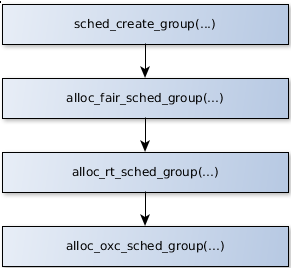
\includegraphics[height=0.25\textheight,width=0.5\textwidth]{images/tg_creation_oxc}
        \caption{The creation of a task group in oxc enabled Linux}
        \label{fig:tg_creation_oxc}
\end{figure}

Corresponding to case 1, now when a task group is created, there 
will be a initilization routine for oxc scheduling. A sketch is shown in 
figure \ref{fig:tg_creation_oxc}. The details of this routinue 
\texttt{alloc\_oxc\_sched\_group} is shown below. 

\begin{lstlisting}[language=C,
        caption={OXC scheduling related initilization 
					during task group creation}]
int alloc_oxc_sched_group(struct task_group *tg, struct task_group *parent)
{
        int i;

        tg->hyper_oxc_rq = parent->hyper_oxc_rq;
        if( parent->hyper_oxc_rq) {
                for_each_possible_cpu(i) {
#ifdef CONFIG_FAIR_GROUP_SCHED
                        tg->cfs_rq[i]->rq =
                                &tg->hyper_oxc_rq->oxc_rq[i]->rq_;
                        if( !parent->se[i] && tg->se[i])
                                tg->se[i]->cfs_rq =
                                      &tg->hyper_oxc_rq->oxc_rq[i]->rq_.cfs;
#endif
#ifdef CONFIG_RT_GROUP_SCHED
                        tg->rt_rq[i]->rq =
                                &tg->hyper_oxc_rq->oxc_rq[i]->rq_;
                        if( !parent->rt_se[i] && tg->rt_se[i])
                                tg->rt_se[i]->rt_rq =
                                       &tg->hyper_oxc_rq->oxc_rq[i]->rq_.rt;
#endif
                }
                tg->oxc_label = 100;
        }
        else
                tg->oxc_label = 0;

        return 1;
}
\end{lstlisting}

The \texttt{alloc\_oxc\_sched\_group} handles oxc related initialization when a 
new task group is created. At first, the a newly created task group will inherit
its parent task group's hyper container. If the parent is an oxc task group, 
this child task group will be directed to per oxc runqueues contained in the
hyper oxc; the result corresponds to the end part of a scheduling route.  
And the \texttt{oxc\_label} for such a child oxc task group is 100.

Case 2 and 3 actually happen at the same time. When explicitly putting the 
parent group inside a hyper ox container, the dscendant task groups will also 
be directed to this hyper oxc. Two methods \texttt{init\_tg\_cfs\_entry\_oxc} and
\texttt{init\_tg\_rt\_entry\_oxc} will be involved in this procedure to 
associate task groups with the hyper ox container. 
The structure in the two is silimar. As an example, Here we only study how the 
CFS part of a task group is handled through \texttt{init\_tg\_cfs\_entry\_oxc}.

\begin{lstlisting}[language=C, caption={To explicitly direct a task group 
						(CFS part) to an OXC \\
					\indent\hspace{5cm} local runqueue}]
static void init_tg_cfs_entry_oxc(struct task_group *tg,
					struct cfs_rq *cfs_rq,
					struct sched_entity *se, int cpu,
					struct sched_entity *parent,
					struct oxc_rq *oxc_rq)
{
	struct rq *rq = rq_of_oxc_rq(oxc_rq);
	init_tg_cfs_entry(tg, cfs_rq, se, cpu, parent);
	tg->cfs_rq[cpu]->rq = rq;
	if( !parent && se)
		se->cfs_rq = &rq->cfs;
} 
\end{lstlisting}
A brief explanation on the parameters:
\begin{itemize}
\item \texttt{tg} is the task group to be dealt with.
\item \texttt{cfs\_rq} is the CFS runqueue that this task group 
		owns. 
\item \texttt{se} is the CFS entity that represents \texttt{tg}.
\item \texttt{cpu} specifies the cfs\_rq pointer inside \texttt{tg} that
		will be redirected. The function 
		\texttt{init\_tg\_cfs\_entry\_oxc}
		redirects one CFS runqueue inside a \texttt{tg} to an oxc 
		runqueue, \texttt{oxc\_rq}, in each call. A hyper ox 
		container can have more than one oxc runqueues inside
		and \texttt{tg} has multiple CFS runqueues too.
		To relate a task group with a hyper ox container requires 
		the \texttt{init\_tg\_cfs\_entry\_oxc} be called multiple times.
\item \texttt{parent} points to the parent CFS scheduling entity.
\item \texttt{oxc\_rq} contains the destinated runqueue. 
\end{itemize}

As for codes, first \texttt{rq\_of\_oxc\_rq} returns the oxc local runqueue.
The mainline kernel method \texttt{init\_tg\_cfs\_entry} is then called to 
re-initialize CFS related work for \texttt{tg}. 
%This is a mainline Linux kernel function called in
%task group creation if CFS group scheduling is set.
The real bridging point is in the following line where 
\texttt{tg} connects its local \texttt{cfs\_rq} on 
\texttt{cpu} to the per oxc runqueue just got. After 
\texttt{init\_tg\_cfs\_entry\_oxc} is invoked over every CPU for the 
task group, CFS tasks and task groups under \texttt{tg} will work in 
the scheduling route leading them to an oxc local runqueue. When a task 
group is explicitly directed to a hyper ox container, the whole family of 
task groups under it will also be associated with this hyper ox container. 
This task group will be the top of this hierarchy, and it will be enqueued 
in the per oxc runqueue's embedded CFS runqueue directly. The last 
\texttt{if} condition returns true when \texttt{tg} is top in the oxc 
group hierarchy.
%One amazing feature of this procedure to relate a task group to a per oxc 
%runqueue is that it has nothing to do tasks under this group.

\section{Run tasks under OXC scheduling framework\label{sec:run}}

As long as per oxc runqueue joins the scheduling route, modular schedulers
can handle tasks in an ox container without differentiating oxc tasks from
non oxc tasks.
%the scheduling 
%of tasks is compatible with modular schedulers in Linux. 
In case to schedule an oxc task, just pass the task itself and its oxc 
local runqueue, instead of per CPU runqueue, to its corresponding 
scheduling class. The local runqueue of an oxc task can be easily tracked 
along the scheduling route. And the scheduler will behave as usual. That 
is, this oxc scheduling framework is transparent to both schedulers and 
tasks.

Because we consider reserving CPU bandwidth for an ox container, there
are scheduling operations that before or after passing parameters to them,
the reservation information should be updated. For these kinds of scheduling
operations, we adapt a relaying mechanism. The parameter is first passed to
another function and after necessary actions, the scheduling operation is
called inside this function. We say that such scheduling operations are
encapsulated in oxc (scheduling) functions.
Still scheduling details for a task are not the framework's work. 

In order to fulfil real time guarantee, oxc tasks are always privileged
to non oxc tasks. Among oxc tasks inside a container, the priority relation
is the same as in Linux. The ox container itself can be considered as a 
virtual Linux system.

For each scheduling operation defined in \texttt{struct sched\_class},
there are three fates for them under oxc scheduling framework: 
some are encapsulated inside oxc functions so as to work with oxc tasks; 
some can work under the framework directly; and others are not supported. 
The table~\ref{tab:op_classes} displays the three classes of scheduling 
operations. The naming convention for oxc functions which encapsulate 
a scheduling operation inside is appending the original name with 
\texttt{\_oxc}. For example, the scheduling operation
\texttt{task\_tick} is called inside in \texttt{task\_tick\_oxc}.
The enqueue and dequeue are two exceptions, they are enclosed in 
\texttt{enqueue\_task\_oxc} and \texttt{dequeue\_task\_oxc}.

\begin{table}[thbp]
  \centering
  \begin{tabular}{l|l|l}\hline
	\small{Work inside an oxc function} & \small{Work without encapsulation} & \small{Unsupported}\\\hline
		check\_preempt\_curr	& yield\_task				& Others	\\
		pick\_next\_task	& yield\_to\_task			&		\\
		put\_prev\_task		& task\_waking				&		\\
		set\_curr\_task		& task\_woken				&		\\
		task\_tick		& set\_cpus\_allowed			&		\\
		enqueue\_task\_rq	& task\_fork				&		\\
		dequeue\_task\_rq	& switched\_from			&		\\
					& switched\_to				&		\\
					& prio\_changed				&		\\
					& get\_rt\_interval			&		\\
					& task\_move\_group			&		\\\hline
  \end{tabular}	
  \caption{The way to handle a scheduling operation under the oxc framework}
  \label{tab:op_classes}
\end{table}

The following will be descriptions on oxc functions with emphasis on ones that
encapsulate a scheduling operation inside.

\subsection{To obtain the runqueue of a task\label{sec:rq_of_task}}
A method \texttt{rq\_of\_task}, listing~\ref{lst:rq_of_task}, is used to 
obtain the runqueue of a task. The runqueue retuned can be an oxc local 
runqueue or per CPU one depending that whether the task is inside a 
container. This function can be used to replace the \texttt{task\_rq} 
macro under oxc framework. For any task, it has both CFS scheduling 
entity and RT entity. And the RT and CFS scheduling routes both exists 
for a task. Here, we exploit the CFS scheduling route. Given 
\texttt{CONFIG\_FAIR\_GROUP\_SCHED} is set or not, the corresponding 
scheduling route is explored to track the runqueue.

\begin{lstlisting}[language=C, 
		caption={Codes to obtain the runqueue of a task},
			label={lst:rq_of_task}]
struct rq* rq_of_task(struct task_struct *p)
{
	struct rq *rq;

#ifdef CONFIG_FAIR_GROUP_SCHED
	rq = p->se.cfs_rq->rq;
#else
	rq = task_rq_fair_oxc(p);
#endif
	return rq;
}
\end{lstlisting}

One important use of this function is in \texttt{oxc\_rq\_of\_task}, 
which takes a task as the input, and returns the ox container the 
task is inside. In case the input is not an oxc task, 
\texttt{NULL} will be returned. The \texttt{oxc\_rq\_of\_task} is 
one most often invoked method under oxc framework. It first gets a 
task's runqueue using the \texttt{rq\_of\_task}, then obtains the ox 
container the runqueue is in, in case the runqueue is in an container.

\subsection{To enqueue an oxc task\label{sec:enqueue_task_oxc}}

When an oxc task arrives, besides enqueue it in the oxc local runqueue,
the ox container's reservation information may be updated if necesary.
The \texttt{enqueue\_task\_oxc} shows the typical scheme for oxc 
functions to enclose a scheduling operation.

\begin{lstlisting}[language=C, 
		caption={To enqueue an task into the oxc local runqueue}]
void enqueue_task_oxc(struct rq *rq, struct task_struct *p, int flags)
{
	struct oxc_rq *oxc_rq = oxc_rq_of_task(p);
	struct rq *rq_ = rq_of_oxc_rq(oxc_rq);

	/* Update the local runqueue' clock. */
	update_rq_clock(rq_);

	/*	
	* Enqueue the task into the local runqueue
	* by its scheduling class.
	*/
	p->sched_class->enqueue_task(rq_, p, flags);

	inc_oxc_tasks(p, oxc_rq);
	enqueue_oxc_rq(oxc_rq);
}
\end{lstlisting}

The method \texttt{oxc\_rq\_of\_task} tracks the scheduling route and 
returns the ox runqueue of an oxc task. Then the ox container's local 
runqueue's time information is updated. Although the ox container does 
not care about scheduling details of tasks inside it, tasks are indeed 
enqueued in its local runqueue and may rely the runqueue's time information. 
We can see that all scheduling details are carried out by a task's 
scheduling class as the \texttt{enqueue\_task} operation of the 
scheduling class is called with the task and local runqueue as inputs. 
The \texttt{inc\_oxc\_tasks} method simply increases the number of oxc 
tasks in the oxc runqueue by one. The reason that such a simple function 
is stiil kept is that as the framework grows more complex in the future, 
extra operations can be put in this method.

\begin{lstlisting}[language=C, 
		caption={To update the number of tasks inside a container} ]
static inline void 
inc_oxc_tasks(struct task_struct *p, struct oxc_rq *oxc_rq)
{
        oxc_rq->oxc_nr_running ++;
}
\end{lstlisting}

Until now, the oxc task has been put in the local runqueue. 
If before the arrival of this task the ox container is empty and not 
throttled, it is time to put this container in its EDF tree.
This is the work of \texttt{enqueue\_oxc\_rq} method. 

\begin{lstlisting}[language=C, 
		caption={To put an ox container in the EDF tree
					if necessary}]
static void enqueue_oxc_rq(struct oxc_rq *oxc_rq)
{
        int on_rq;

        on_rq = oxc_rq_on_rq(oxc_rq);

        BUG_ON(!oxc_rq->oxc_nr_running);
        BUG_ON(on_rq && oxc_rq_throttled(oxc_rq));

        if( on_rq) {
                /* Already queued properly. */
                return;
        }
        /* We do not put a throttled oxc_rq in the edf tree. */
        if( oxc_rq_throttled(oxc_rq))
                return;

        oxc_rq_update_deadline(oxc_rq);
        __enqueue_oxc_rq(oxc_rq);
}
\end{lstlisting}

\texttt{on\_rq} tells if the container \texttt{oxc\_rq} is in a edf tree.
\texttt{BUG\_ON} is a Linux kernel macro. If the condition it checks is 
\texttt{true}, then the kernel will crash! Because we just put a task
in the local runqueue, so the first \texttt{BUG\_ON} should be passed.
When an ox container runs out of its budget, it should be moved from the
edf tree, this is what the second \texttt{BUG\_ON} checks. Now we pass
the two \texttt{BUG\_ONs}. If the \texttt{oxc\_rq} is already on edf 
tree or moved from the tree because of exhausting budget, nothing needs 
to be done. There are two conditions for an ox container to be outside
an edf tree: it is throttled or it is empty. If the last \texttt{if}
condition is passed, this means a task just joins an empty container. 
Recall the CBS rules ''when a task arrives and the server is idle, update 
the deadline if necessary''. This is exactly what 
\texttt{oxc\_rq\_update\_deadline} does. When it comes to CPU reservation,
an ox container corresponds to a constant bandwidth server in CBS theory.
\texttt{\_enqueue\_oxc\_rq} is a quite mechanical procesure to put an
oxc runqueue in an edf tree.

\subsection{To dequeue an oxc task\label{sec:dequeue_task_oxc}}

\texttt{dequeue\_task\_oxc} is the opposite method of 
\texttt{enqueue\_oxc\_rq}.

\begin{lstlisting}[language=C, 
		caption={To remove a task from the oxc local runqueue}]
static void 
dequeue_task_oxc(struct rq *rq, struct task_struct*p, int flags)
{
        struct rq *rq_ = rq_of_task(p);
        struct oxc_rq *oxc_rq = container_of(rq_, struct oxc_rq, rq_);

        /* Update the local runqueue. */
        update_rq_clock(rq_);
        /*
         * Dequeue the task from the local runqueue 
         * by its scheduling class.
         */
        p->sched_class->dequeue_task(rq_, p, flags);

        dec_oxc_tasks(p, oxc_rq);
        dequeue_oxc_rq(oxc_rq);
}
\end{lstlisting}

The layout inside \texttt{dequeue\_task\_oxc} is the same as what we see in
\texttt{enqueue\_task\_oxc}: local runqueue's clock information is updated,
local runqueue and task are relayed to the corresponding scheduler, 
the task number and EDF tree are updated. When an oxc task leaves the 
container, it is the time to check if the oxc is empty or not, which is 
done in \texttt{dequeue\_oxc\_rq}.

\begin{lstlisting}[language=C,
		caption={To remove an ox container 
				from the EDF tree if necessary}]
static void dequeue_oxc_rq(struct oxc_rq *oxc_rq)
{
        int on_rq;

        on_rq = oxc_rq_on_rq(oxc_rq);
        /*
         * Here we do not expect throttled oxc_rq to be in the 
         * edf tree. Note that when an oxc_rq exceeds its 
         * maximum budget, it is dequeued via 
         * sched_oxc_rq_dequeue().
         */
        BUG_ON(on_rq && oxc_rq_throttled(oxc_rq));
        /* 
         * If an oxc_rq is not in the edf tree, it should 
         * be throttled or have no tasks enqueued.
         */
        BUG_ON(!on_rq && !oxc_rq_throttled(oxc_rq) && !oxc_rq->oxc_nr_running);

        if( on_rq && !oxc_rq->oxc_nr_running) {
                /* Dequeue the oxc_rq if it has no tasks. */
                __dequeue_oxc_rq(oxc_rq);
                return;
        }
}
\end{lstlisting}

The comments are explanable enough. \texttt{\_\_dequeue\_oxc\_rq} 
is the counterpart of \texttt{\_\_enqueue\_oxc\_rq} to remove an oxc
runqueue from the EDF tree.

\subsection{To check the preemption condition
			\label{sec:check_preempt_curr_oxc}}
When a task wakes up from sleeping or is created, the scheduler will check 
if it can preempt temporarily running task in the same CPU. If the current 
task is an oxc task and the waking task is not an oxc task, the later 
cannot preempt the current one. If both are non oxc tasks, Linux already 
has methods to check. So here we only pay attention to the situation
when the waking task is an oxc task.

\begin{lstlisting}[language=C, 
		caption={The preemption check for an oxc task},
		label={lst:check_preempt_curr_oxc}]
static inline int
check_preempt_oxc_rq(struct task_struct *curr, struct task_struct *p, int flags)
{
        struct oxc_rq *oxc_rq = oxc_rq_of_task(p);
        struct oxc_rq *oxc_rq_curr = oxc_rq_of_task(curr);
        const struct sched_class *class;

        if(oxc_rq_throttled(oxc_rq)
              return 0;
        /* 
         * Tasks from a unthrottled oxc_rq always has a higher 
         * priority than non oxc tasks.
         */
        if( !oxc_rq_curr)
                return 1;

        /* Both p and current task are in the same oxc_rq. */
        if( oxc_rq_curr == oxc_rq) {
                if( p->sched_class == curr->sched_class) 
                        curr->sched_class->check_preempt_curr(
                                      &oxc_rq->rq_, p, flags);
                else {
                        for_each_class(class) {
                                if( class == curr->sched_class)
                                        break;
                                if( class == p->sched_class) {
                                        resched_task(curr);
                                        break;
                                }
                        }
                }

                return 0;
        }

        /* 
         * p and current tasks are oxc tasks from 
         * different ox containers. 
         */
        return oxc_rq_before(oxc_rq, oxc_rq_curr);
}
\end{lstlisting}

\texttt{curr} and \texttt{p} are the current task and waking task 
respectively. If task \texttt{p}'s container is throttled, it cannot 
preempt currently running task. Otherwise, if \texttt{curr} is not an 
oxc task, the privilege is given to oxc task \texttt{p}.
When both \texttt{p} and \texttt{curr} are oxc tasks and are contained 
in the same oxc runqueue: if they are even in the same scheduling class, 
it's the modular scheduler's responsibility to decide if a preemption 
can happen or not; otherwise, the task whose scheduling class has higher 
priority in the scheduler chain is chosen to run. In the last case, they 
two are from different ox containers. Now, \texttt{oxc\_rq\_before} 
checks if a contaienr's deadline is before another's deadline. The one 
with earlier deadline will run. 

\subsection{To pick up an oxc task\label{sec:pick_next_task_oxc}}

When to pick a most eligible task to run in a system, oxc tasks should 
be checked first. If there is no eligible oxc tasks, then non oxc tasks 
are considered. \texttt{pick\_next\_task\_oxc} is responsible for choosing 
the most eligible oxc task in a CPU.

\begin{lstlisting}[language=C, label={lst:pick_next_task_oxc},
		caption={To pick up the most eligible oxc task}]
static struct task_struct* pick_next_task_oxc(struct rq *rq)
{
        struct oxc_rq *oxc_rq;
        struct rq *rq_;
        struct task_struct *p, *curr;
        const struct sched_class *class;
        /* This clock update is necessary! */
        update_rq_clock(rq);
        update_curr_oxc_rq(rq);
        oxc_rq = pick_next_oxc_rq(rq);
        if( !oxc_rq)
                return NULL;

        rq_ = rq_of_oxc_rq(oxc_rq);

        update_rq_clock(rq_);

        for_each_class(class) {
                if( class != &idle_sched_class) {
                        p = class->pick_next_task(rq_);
                        if( p) {
                                rq_->curr = p;
                                return p;
                        }
                }
        }

        return NULL;
}
\end{lstlisting}

Inside the oxc function \texttt{pick\_next\_task\_oxc},
there is one thing to note: not only local runqueue's clock
is updated, but also the per CPU runqueue's clock is updated here.
This is because the reservation time of an ox container is counted
using the per CPU runqueue's clock and to keep the clock on time
for the container's use, here it is updated. 
\texttt{pick\_next\_oxc\_rq} is called to pick the ox runqueue with the 
earliest deadline in a CPU. Then along the scheduling class chain, each
scheduler uses its scheduling operation trying to find the most eligible
task in the ox container's local runqueue. A very important method here 
is \texttt{update\_curr\_oxc\_rq}. The budget comsumption of an ox 
container actually happens in this method.

\begin{lstlisting}[language=C, 
		caption={To update an ox container's runtime information}]
static void update_curr_oxc_rq(struct rq *rq)
{
        struct task_struct *curr = rq->curr;
        struct oxc_rq *oxc_rq = oxc_rq_of_task(curr);
        u64 delta_exec;
        /*
         * If current task is not oxc task, simply return.
         */
        if( !oxc_rq)
                return;

        delta_exec = rq->clock - oxc_rq->oxc_start_time;
        oxc_rq->oxc_start_time = rq->clock;
        if( unlikely((s64)delta_exec < 0))
                delta_exec = 0;

        raw_spin_lock(&oxc_rq->oxc_runtime_lock);

        oxc_rq->oxc_time += delta_exec;
        if( sched_oxc_rq_runtime_exceeded(oxc_rq)) {
                resched_task(curr);
        }

        raw_spin_unlock(&oxc_rq->oxc_runtime_lock);
}
\end{lstlisting}

\texttt{update\_curr\_oxc\_rq} updates the runtime value of 
an oxc runqueue. If the budget in current period is exhausted, the
current task needs to be rescheduled. the local spinlock 
\texttt{oxc\_runtime\_lock} protects the update of runtime from
interleave. The \texttt{sched\_oxc\_rq\_runtime\_exceeded} is
used to check if the ox container has exceeded its budget in a
period.

\begin{lstlisting}[language=C, 
	caption={To check if an ox container should be throttled}]
static int sched_oxc_rq_runtime_exceeded(struct oxc_rq *oxc_rq)
{
        u64 runtime = sched_oxc_rq_runtime(oxc_rq);
        u64 period = sched_oxc_rq_period(oxc_rq);

        /* 
         * If the runtime is set as 'RUNTIME_INF',
         * the ox container can run without throttling.
         */
        if( runtime == RUNTIME_INF)
                return 0;

        /* 
         * If the runtime to be larger the the period,
         * the ox container can run without throttling.
         */
        if( runtime >=period)
                return 0;

        /* There is still budget left. */
        if( oxc_rq->oxc_time < runtime)
                return 0;
        /* 
         * The reservation in a period has been exhausted,
         * to set the throttling label, remove the oxc_rq
         * from the edf tree and start the recharging timer.
         */
        else {
                oxc_rq->oxc_throttled = 1;
                sched_oxc_rq_dequeue(oxc_rq);
                start_oxc_period_timer(oxc_rq);

                return 1;
        }
}
\end{lstlisting}

Inside \texttt{sched\_oxc\_rq\_runtime\_exceeded}, at first
a series of non exceeded conditions is checked, which is 
easy to understand. The last \emph{else} statement deals with
the case that the container should be throttled: the 
\texttt{oxc\_throttled} label is set, the oxc runqueue is removed 
from the edf tree and the timer is set to fire at the current 
deadline, \texttt{oxc\_deadline}, to recharge the budget.

\subsection{put\_prev\_task\_oxc\label{sec:put_prev_task}}

The scheduling operation \texttt{put\_prev\_task} is called when 
the currently running task is possible to be replaced. It performs some 
conclusion work for the task. Although the currently running task may 
keep running without giving up the CPU. If currently running task is an 
oxc task, when \texttt{put\_prev\_task} is called, this is also a point 
to update the ox container runtime information. 

\begin{lstlisting}[language=C, label={lst:put_prev_task_oxc},
		caption={Conclusion work before an oxc task is switched 
				out of a CPU}]
static void 
put_prev_task_oxc(struct rq* rq, struct task_struct *p)
{
        struct rq *rq_ = rq_of_task(p);

        update_rq_clock(rq_);
        update_curr_oxc_rq(rq);

        p->sched_class->put_prev_task(rq_, p);
}
\end{lstlisting}

Now, when a \texttt{put\_prev\_task} operation is needed and the
currently running task is an oxc task, instead of calling the 
\texttt{put\_prev\_task} defined in a scheduling class directly, our
\texttt{put\_prev\_task\_oxc} encapsulation will be called first then
ox container local runqueue and current task will be relayed to
the corresponding scheduler.

\subsection{set\_curr\_task\_oxc\label{sec:set_curr_task_oxc}}
%The scheduling operation \texttt{put\_prev\_task} is the last scheduling 
%operation before a task gives up a CPU (of course, if it is chosen again 
%immediately, it can still occupy the CPU). 
The \texttt{put\_prev\_task}/\texttt{set\_curr\_task} is used whenever
the current task is changing policies or groups. Similiar as what happens 
to \texttt{put\_prev\_task}, there is an oxc function 
\texttt{set\_curr\_task\_oxc} that performs the operation 
\texttt{set\_curr\_task\_oxc} inside and start an ox container's
budget counting.

\begin{lstlisting}[language=C,
	caption={Another point to update reservation information},
	label={lst:set_curr_task_oxc}]
static void set_curr_task_oxc(struct rq *rq)
{
        struct task_struct *curr = rq->curr;
        struct rq *rq_ = rq_of_task(curr);
        struct oxc_rq *oxc_rq;

        oxc_rq = container_of(rq_, struct oxc_rq, rq_);

        oxc_rq->oxc_start_time = oxc_rq->rq->clock;

        update_rq_clock(rq_);
        curr->sched_class->set_curr_task(rq);
}
\end{lstlisting}

One thing to note in listing~\ref{lst:set_curr_task_oxc} is that 
this time the per CPU runqueue parameter is passed to the 
task's corresponding scheduling class. First of all, this is feasible 
because \texttt{set\_curr\_task} operation updates the infomation in the 
scheduling route excluding the runqueue (at least in scheduling classes
in mainline Linux) and the current task in the per CPU runqueue
and current task in the earliest dealine oxc runqueue are the same one. 
So, there is no difference to pass which runqueue. 
The real reason is that there is a possible insconsistent state under 
current oxc framework. Initially, the current task in an ox 
container's local runqueue is 
NULL\footnote{This will be improved in future work}, which is different
from the per CPU runqueue's behaviour that the default current task would 
be the special idle task from scheduling class \texttt{sched\_idle}. 
At this time, if the current task is moved 
into this ox container, the \texttt{set\_curr\_task} operation is called 
even before the task is really enqueued into the container's local runqueue. 
That is, the current task in the local runqueue is still \texttt{NULL} when
\texttt{set\_curr\_task} is called and this will cause problems. Thus, a 
per CPU runqueue is used here temporarily.

\subsection{task\_tick\_oxc\label{sec:task_tick_oxc}}

The \texttt{task\_tick} operation is the most frequently called 
scheduling operation and is used to update the task's timing 
information. 
The oxc control also utilizes this opportunity to update the 
current ox container's runtime information and 
local runqueue when the CPU is occupied by an oxc task.

\begin{lstlisting}[language=C, label={lst:task_tick_oxc},
		caption={The most frequently called entry to update a container's runtime}]
			
static void 
task_tick_oxc(struct rq *rq, struct task_struct *p, int queued)
{
        struct rq *rq_ = rq_of_task(p);

        update_curr_oxc_rq(rq);
        update_rq_clock(rq_);

        p->sched_class->task_tick(rq_, p, queued);
}
\end{lstlisting}

\section{SMP support in oxc framework}
An ox container based scheduling system acts with no difference as the 
per CPU scheduling system. Inside different ox containers, the 
scheduling is performed independently and a group of ox containers
can be arranged in one hyper container to realize multi-processor 
bandwidth reservation. For a hyper ox container, tasks are partitioned 
to each ox container and task migration or load balancing between 
different ox contaienrs in a hyper container are missing now.

\section{User interfaces provided by OXC framework}
Currently, the user interfaces, mainly for test purposes, 
of oxc framework are based on cgroup virtual
filesystem. The CPU reservation functionality is realized through 
\emph{cpu} cgroup subsystem. This \emph{cpu} cgroup subsystem is for CPU 
bandwidth control in Linux. RT throttling, CFS group scheduling and 
CFS bandwidth control are all realized through it. The following demonstrates 
how to use the oxc framework. The hardware platform is assumed to have dual
processors.\\
To mount the \emph{cpu} cgroup subsystem(in directory /cgroup):
\begin{lstlisting}
	#mount -t cgroup -ocpu none /cgroup
\end{lstlisting} 
To create a cgroup for CPU reservation :
\begin{lstlisting}
	#mkdir -p /cgroup/cg
\end{lstlisting}
Observe the files inside \texttt{/cgroup/cg} directory, there is one
new file named \texttt{cpu.oxc\_control} and it is the interface to control
CPU bandwidth in oxc framework. However, if one tries to see the content
of this file:
\begin{lstlisting}
	#cat /cgroup/cg/cpu.oxc_control
\end{lstlisting}
It will display nothing. This is because by default the oxc reservation
is disabled until the reservation is triggered for the first 
time. The reservation is triggerred by setting reservation parameters.
To reserve bandwidth in a CPU, three parameters should be specified:
\texttt{CPU number, maximum budget and period}. For example:
\begin{lstlisting}
	#echo 0 100000/1000000 1 20000/500000 > cg/cpu.oxc_control
\end{lstlisting}
This command reserve 100ms every 1s on CPU 0 and 20ms every 500ms on CPU 1
to cgroup \texttt{cg}. 0 and 1 are CPU numbers. 100000 and 20000 are maximum
budgets and 1000000 and 500000 are periods. 
In fact, behind this command, a hyper ox container with two ox containers
inside is created. 
Tasks and task groups inside cgroup \texttt{cg} and its
descedant will be work inside these two ox containers since now.
The two containers' reservation parameters are specified
by the command inputs. 
The unit for budget and period value in the command 
is micro second. This follows the convention in \emph{cpu} cgroup
subsystem, since when you use other bandwidth control mechanisms the value 
is also considered in micro seconds. Tasks inside this cgroup and its further 
sub cgroups will run using the above reserved CPU bandwidth. Now we can say 
\texttt{cg} is contained in a hyper ox container.

Now to \texttt{cat} the content of the \texttt{cpu.oxc\_control} interface 
under directory \texttt{/cgroup/cg}:
\begin{lstlisting}
	#cat /cgroup/cg/cpu.oxc_control
\end{lstlisting}
The reservation parameters we just set will be displayed:
\begin{lstlisting}
	0 100000/1000000 1 20000/500000
\end{lstlisting}
So the file \texttt{oxc\_control} is an interface used for both setting up
and displaying reservation parameters. Reservation parameters can be 
configured in the same way as they are initially set. Furthermore,
there is no need to set up or configure reservation parameters for two 
CPUs at the same time. Suppose in some point, users decide to decrease 
the reservation from CPU 1, they can simply use the following command to
operate on CPU 1 onlu.
\begin{lstlisting}
	#echo 1 20000/1000000 > cg/cpu.oxc_control
\end{lstlisting}
The reservation on CPU 1 is dereased to 20ms every 1s and the reservation
on another CPU is not interfered. 

To create a sub cgroup for cgroup \texttt{cg}:
\begin{lstlisting}
	#mkdir -p /cgroup/cg/cg_0
\end{lstlisting}
The cgroup \texttt{cg\_0} is contained in the same hyper container as
its parent. Try to \texttt{cat} the \texttt{cpu.oxc\_control} file in 
this sub cgroup: 
\begin{lstlisting}
	#cat /cgroup/cg/cg_0/cpu.oxc_control
\end{lstlisting}
An error message will be returned. This is because for a cgroup family
contained in a hyper container, only the top cgroup is allowed for people
to browse and modify reservation parameters.

People can move tasks to cgroup \texttt{cg} and \texttt{cg\_0}. For example
\begin{lstlisting}
	#echo 1982 > cg/tasks
	#echo 1983 > cg_0/tasks
\end{lstlisting}
This moves task with \texttt{pid} 1982 and 1983 to cgroup \texttt{cg} and
\texttt{cg\_0} respectively. Tasks can be RT tasks or normal tasks. All 
tasks inside an ox container behave as working on a virtual Linux system
and utilize the reserved bandwidth.
% Note here we use ''ox container'', not
%''hyper ox container'', because in temporary iplementation, tasks inside
%a hyper ox container are partitioned into each ox containers. 

The oxc tasks can move between different cgroups contained in the same 
hyper container. They can move between ox containers and hyper containers.
They can also leave an ox container and return to be a non oxc task.

Until now, how to reserve CPU bandwidth under oxc framework is introduced.
Now let's see how to distribute the reserved CPU power.
ALthough users cannot browse reservation parameters in cgroup
\texttt{cg\_0}, they can indeed set reservation parameters for 
\texttt{cg\_0}, which will trigger reserved power redistribution.
\begin{lstlisting}
	#echo 0 100000/2000000 1 20000/1000000 > cg/cpu.oxc_control
\end{lstlisting}
After this, a new hyper container with reservation parameters
1000000/1500000 on CPU 0 and 20000/1000000 on CPU 1 will be created
and \texttt{cg\_0} and its descendant cgroups will be associated with
it. Now, although \texttt{cg} and \texttt{cg\_0} are still in the same
hierarchy through the cgroup directory observation, they are indeeded 
contained in two different hyper containers.
The ideal semantics of the above command should also include that the 
reserved bandwidth by \texttt{cg} need to be decreased the same vaue as 
distributed to \texttt{tg\_0}. This behaviour is still missing in current 
prorotype implementation of oxc framework. Yet this is indeed implementable.
Also, the total reserved bandwidth in the system should not be more one in
each CPU; this condition test is not realized either.

\section{Cooperation with scheduling mechanisms inside Linux}

First let's discuss a simple case is when both
\texttt{CONFIG\_FAIR\_GROUP\_SCHED} and \texttt{CONFIG\_RT\_GROUP\_SCHED} 
are not set; that is, task grouping is not 
enabled. In this case, oxc tasks share the reserved CPU bandwidth directly
according to their scheduling policies. In fact, in this situation, the oxc 
control can be used to repeat RT throttling and CFS bandwidth control. 
However, at this time, the reservation is in a real time way and is more 
flexible since CPU bandwidth from different CPUs can be different under 
oxc framework. The result of IRMOS real time scheduler can also be achieved 
by our framework. Consider future scheduling classes that are possible to 
be merged in Linux kernel. For example the \texttt{schedule\_deadline} 
patch, which does not have task grouping scheme by itself. 
Not only that it can work with oxc scheduling naturally becaue of the
ox container's ''open-to-entension'' feature, but also the oxc framework 
can utilize cgroup virtual filesystem as a way to group deadline tasks. 

When the kernel compilation option \texttt{CONFIG\_FAIR\_GROUP\_SCHED} is set, 
the CFS task group scheduling is enabled. Task groups inside the same hyper ox 
container follow the rules of CFS grouping and share the reserved CPU power. 
CFS group scheduling is applied in different areas independently: 
each hyper ox container is an area and outside all ox containers there
is an area. 
%Inside one hyper ox container, bandwidths are reserved
%and task groups inside this hyper ox container share the reserved 
%computation power according to the fairness task group scheduling rules. 

When \texttt{CONFIG\_RT\_GROUP\_SCHED} is set, RT throttling is enabled.
It's necessary to first analyze the possible result when RT throttling 
is applied in a hyper ox container. Suppose inside an container, $Q/T$ 
is the bandwidth reserved from the CPU and RT throttling sets parameters as 
$Q^{'}/T^{'}$ and $Q^{'}/T^{'} \le Q/T$. The ideal behaviour for such an
ox container would be : the container distributes reserved CPU power 
to tasks inside it; and RT tasks inside a container will be throttled when
$Q^{'}$ units of CPU cycles are exhausted in a period $T^{'}$, then non
RT tasks in this container can run. However, in real world a coarse 
combination could cause unreliable results . For example, 
$Q^{'}/T^{'} = 1/10$ and $Q/T = 10/50$. It can happen that there are other 
higher priority containers in the same CPU and in one period the example 
container get the right to use the CPU on the last 10 units of CPU cycles 
in its period. RT tasks inside this container immediately take over the CPU; 
yet after one unit, they are throttled. So, RT tasks only run 1 unit over 
50 unit of CPU cycles although 10 units are reserved. The RT throttling 
result inside a hyper ox container is not stable. Even if we set the period 
parameter in RT throttling the same as its container's, because that RT
throttling and oxc control use different timers, there is a unsynchronization 
between them and can lead to still complex situations.

In a statement, to apply RT throttling naively inside an ox container 
is not efficient. One possible solution is to count the time 
consumption in RT throttling using the ox container's timer, 
this basically means to implement a copy of RT throttling in oxc 
framework itself. In such a case, if some constraints are put, like
the RT throttling period should equal to the container's period, 
we can expect predictable behaviour. Another solution is simply disable 
RT throttling inside an ox container, because oxc scheduling framework 
itself can perform the same result in a real time way as RT throttling. 
In current implementation, there is no communication between RT throttling
and oxc control. And when \texttt{CONFIG\_RT\_GROUP\_SCHED} is set, the 
result is not satisfiable.

The test between CFS bandwidth and oxc control is not conducted yet.
If \texttt{CONFIG\_CFS\_BANDWIDTH} is set, we expect that the situation 
could be similiar to what we see in RT throttling case.

Among cgroup subsystems, there is one \texttt{cpuset} subsystem also 
affecting scheduling behaviour in a cgroup.
After \texttt{cpuset} cgroup subsystem is mounted in a cgroup, there is an 
interface \texttt{cpuset.cpus} appearing in the dorectory. This file 
can control which CPU the tasks inside this cgroup can use.
For example, 
\begin{lstlisting}
	#echo 1 > cpuset.cpus
\end{lstlisting}
This will result tasks inside this cgroup can only run on CPU 1.
In oxc scheduling framework, we have the concept of hyper ox container, which 
control the CPUs that tasks inside it can run in. So, this idea is
compatible with \texttt{cpuset} cgroup subsystem. However, until now the two
mechanisms work independently; future work to bridge the two will make 
the system more consistent.

%%% Local Variables: 
%%% mode: latex
%%% TeX-master: "main"
%%% End: 
